%
%--- 
%-----------------------------------
\section{Semiclassical approach}
\label{sec:semiclassical-approach}
%-----------------------------------
%--- 
%

In the previous section, we consider phenomenological rate equations to study two-level atomic transitions. This approach does not contemplate coherence effects nor a fundamental understanding of line broadening mechanisms. In a first attempt, we can take the coherence effects into account assuming the interaction between a classical light field (electromagnetic waves) and an atom whose internal states are described by a quantum state vector $ \ket{\psi} $. Indeed, this is a proper treatment as long as we are only interested in stimulated processes. However, spontaneous emission comes from the interaction between atom and the vacuum modes of the quantized electromagnetic field, an incoherent relaxation process. Therefore, a single state vector is not sufficient to analyze an atom under both stimulated and spontaneous processes since such system is under decoherence. A proper description comes through the density operator, which describes a statistical mixture of quantum states. This approach allows us to study the system time evolution taking both coherent and incoherent processes into account through a master equation. In this section, we shall introduce the density operator formalism to investigate atom-light interaction.

%
%-----------------------------------
\subsection{The density operator}
\label{sec:density-operator}
%-----------------------------------
%

The density operator represents an \textbf{ensemble} of identical systems in different quantum states. Let us consider a system which can be found in a quantum state $ \ket{\psi_k} $ with probability $ P_{k} $. This system is represented by the following density operator
\begin{equation}
	\hat{\rho} \equiv \sum_{k} P_{k} \ketbra{\psi_k}{\psi_k}\ \ \ \ \textrm{so that}\ \ \ \sum_k P_k = 1.
\end{equation}
When the system is described by a single state vector $ \ket{\psi} $, which means $ \hat{\rho} = \ketbra{\psi}{\psi} $, it is said to be in a \textbf{pure state}, otherwise it is said to be in a \textbf{mixed state}.

Let us consider the orthonormal basis $ \{\ket{n} : n \in \{1, 2, \cdots, N\}\} $ on which it is possible to represent the states $ \{\ket{\psi_k}\} $ and the density operator $ \hat{\rho} $ as
\begin{gather}
	\ket{\psi_k} = \sum_{n = 1}^{N} |c_{k,n}|e^{\phi_{k,n}} \ket{n},\ \ 
	\hat{\rho} = \left[ 
	\begin{matrix}
		\rho_{1,1} & \cdots & \rho_{1,N} \\
		\vdots & \ddots & \vdots \\
		\rho_{N,1} & \cdots & \rho_{N,N}
	\end{matrix} \right], \\
	\textrm{where}\ \ \ \rho_{m,n} = \braket{m|\hat{\rho}|n}\ \ \textrm{(matrix elements),}
\end{gather}
being $ \rho $ the \textbf{density matrix} and $ c_{k,n} = |c_{k,n}|e^{\phi_{k,n}} $. From now on, we shall assuming the abuse of notation $ \hat{\rho} = \rho $ in order to make the definion of a density operator easy by using its matrix represantion. The probability of finding a state $ \ket{n} $ in a given state vector $ \ket{\psi_k} $ is $ P_k |c_{k,n}|^2 $. Then the probability of finding the state $ \ket{n} $ in any state vector is
\begin{equation}
	\sum_{k} P_k |c_{k,n}|^2 = \sum_{k} P_k \underbrace{\braket{n|\psi_k}}_{c_{k,n}}\underbrace{\braket{\psi_k|n}}_{c_{k,n}^*} = \bra{n} \left( \sum_k P_k \ketbra{\psi_k}{\psi_k} \right) \ket{n} = \braket{n|\hat{\rho}|n} = \rho_{n,n}.
\end{equation}
Therefore, the diagonal terms, also referred as \textbf{populations}, give the probability of measuring the system in some state $ \ket{n} $, which implies
\begin{equation}
	\Tr[\rho] = \sum_{n = 1}^{N} \braket{n|\hat{\rho}|n} = \sum_{n = 1}^{N} \rho_{n,n} = 1,
\end{equation} 
where $ Tr[\hat{\rho}] $ is the \textbf{trace} of the operator $ \hat{\rho} $. This operation is independent of the basis since it is invariant with respect to any unitary transformation. Moreover, the trace is also invariant under cyclic permutation of the product so that
\begin{equation}
	\Tr[\hat{A}\hat{B}\hat{C}] = \Tr[\hat{B}\hat{C}\hat{A}] = \Tr[\hat{C}\hat{A}\hat{B}].
\end{equation}
The off-diagonal terms are called \textbf{coherences}. They give information about the relative phase of different components. Let us consider a pure state so that
\begin{align}
	\rho_{m,n} &= \bra{m}(\ketbra{\psi}{\psi})\ket{n} = \bra{m}\left(\sum_{p} |c_p|e^{i\phi_p} \ket{p}\right)\left(\sum_{q} |c_q|e^{- i \phi_{q}} \bra{q}\right)\ket{n} \\
	&= \sum_{p,q} |c_p c_q |e^{i(\phi_p - \phi_q)} \braket{m|p} \braket{q|n} = |c_m c_n| e^{i(\phi_m - \phi_n)}
\end{align}
For mixed systems, the coherences will be the sum of complex numbers corresponding to different states $ \ket{\psi_k} $. Furthermore, it is possible to check whether a system is pure or mixed evaluating the quantity $ \Tr[\hat{\rho}^2] $. For a pure state $ \hat{\rho}_{pure} = \ket{\psi}\bra{\psi} $, we have 
\begin{equation}
	\hat{\rho}_{pure}^2 = \ket{\psi}\braket{\psi|\psi}\bra{\psi} = \ketbra{\psi}{\psi} = \hat{\rho}_{pure} \Rightarrow \Tr[\hat{\rho}_{pure}^2] = \Tr[\hat{\rho}_{pure}] = 1.
\end{equation}
Indeed, $ \hat{\rho}_{pure}^n = \hat{\rho}_{pure} $ for any pure state, being $ n $ a non-negative integer. To study the case of a mixed state defined by the density operator $ \hat{\rho}_{mixed} $, let us assume a basis where the matrix $ \rho_{mixed} $ is diagonal so that
\begin{equation}
	\Tr[\rho_{mixed}^2] = \sum_n (\rho_{n,n})^2 \leq \sum_n \rho_{n,n} = 1,
\end{equation}
since $ 0 \leq \rho_{n,n} \leq 1 $. A diagonal pure state has only a single non-zero element, whereas a diagonal mixed state necessarily has more then one non-zero element. Hence, being the trace operation independent of the basis, for a mixed state we always have
\begin{equation}
	\Tr[\hat{\rho}_{mixed}^2] < 1.
\end{equation}

We can also compute expectation values using the trace operation. Let us consider an observable $ \hat{A} $ whose matrix elements are $ A_{m,n} = \braket{m|\hat{A}|n} $. The expectation value $ \braket{\hat{A}} $ is expressed by
\begin{equation}
	\braket{\hat{A}} = \sum_{k} P_k \braket{\psi_k|\hat{A}|\psi_k}.
\end{equation}
On the other side,
\begin{gather}
	\hat{\rho}\hat{A} = \sum_{k} P_k \ketbra{\psi_k}{\psi_k}\hat{A} \Rightarrow \braket{n|\hat{\rho}\hat{A}|n} = \sum_{k} P_k \braket{\psi_k|\hat{A}|n} \braket{n|\psi_k} \Rightarrow \\
	\Rightarrow \Tr[\hat{\rho}\hat{A}] = \sum_{n} \braket{n|\hat{\rho}\hat{A}|n} = \sum_{k} P_k \bra{\psi_k} \hat{A} \underbrace{\left( \sum_{n = 1}^{N} \ketbra{n}{n} \right)}_{\mathbb{I}} \ket{\psi_k} = \sum_{k} P_k \braket{\psi_k|\hat{A}|\psi_k} \\
	\therefore \Tr[\hat{\rho}\hat{A}] = \sum_{k} P_k \braket{\psi_k|\hat{A}|\psi_k} = \braket{\hat{A}}.
	\label{eq:trace-average}
\end{gather}
Therefore, the ensemble average of any observable $ \hat{A} $ can be calculated from the diagonal elements of the operator matrix $ \hat{\rho}\hat{A} $.

The density operator formalism is also great to manage \textbf{composite system}. Let us consider a system $ A $ defined by the density operator $ \hat{\rho}_A $ and the Hilbert space $ \mathcal{H}_{A} $, and a system $ B $ represented by the density operator $ \hat{\rho}_B $ and the Hilbert space $ \mathcal{H}_B $. The total system, which take A and B into account, is described by the density operator $ \hat{\rho}_{AB} $ and the Hilbert Space $ \mathcal{H}_A \otimes \mathcal{H}_B $. The operator $ \hat{\rho_A} $ and $ \hat{\rho_B} $ can be seen as \textbf{reduced density matrices}, which can be derived from $ \hat{\rho}_{AB} $ through the \textbf{partial trace operation},
\begin{equation}
	\hat{\rho}_A = \Tr_{B} [\hat{\rho}_{AB}]\ \ \ \textrm{and}\ \ \ \hat{\rho}_B = \Tr_A [\hat{\rho}_{AB}].
\end{equation}

Let us consider a pure state $ \ket{\psi_{AB}} $ of both system $ A $ and $ B $ given by
\begin{equation}
	\ket{\psi_{AB}} = \sum_{m,n} c_{m,n} \ket{m} \otimes \ket{n},\ \ \textrm{where}\ \ \sum_{m,n} |c_{m,n}| = 1.
	\label{eq:ket-A-B}
\end{equation}
If the systems are \textit{independent}, we can associate a state $ \ket{\psi_A} = \sum a_m \ket{m} $ to the system $ A $ and $ \ket{\psi_B} = \sum b_n \ket{n} $ to the system $ B $ so that
\begin{equation}
	\ket{\psi_{AB}} = \ket{\psi_A} \otimes \ket{\psi_B} = \left( \sum_m a_m \ket{m} \right) \otimes \left( \sum_n b_n \ket{n} \right) = \sum_{m,n} a_m b_n \ket{m} \otimes \ket{n}.
	\label{eq:ket-A-B-independent-systems}
\end{equation}
From equations (\ref{eq:ket-A-B}) and (\ref{eq:ket-A-B-independent-systems}), we obtain $ c_{m,n} = a_m b_n $. Then, the density operator $ \hat{\rho}_{AB} $ is given by
\begin{align}
	\hat{\rho}_{AB} &= \ketbra{\psi_{AB}}{\psi_{AB}} = \sum_{m,n} \sum_{m',n'} a_{m} a_{m'} b_{n} b_{n'} \ketbra{m}{m'} \otimes \ketbra{n}{n'} = \nonumber\\
	&= \left( \sum_{m,m'} a_m a_m' \ketbra{m}{m'} \right) \otimes \left( \sum_{n,n'} b_n b_n' \ketbra{n}{n'} \right) = \nonumber \\ 
	&= \ketbra{\psi_A}{\psi_A} \otimes \ketbra{\psi_B}{\psi_B} = \hat{\rho}_a \otimes \hat{\rho}_B.
\end{align}
Therefore, when two systems $ A $ and $ B $ are \textbf{uncorrelated} or \textit{independent}, we can write the density operator of both systems as a tensor product between the density operator of the system $A $ and the density operator of the system $ B $,
\begin{equation}
	\hat{\rho}_{AB} = \hat{\rho}_A \otimes \hat{\rho}_B.
\end{equation}


%
%-----------------------------------
\subsection{Two-level system and the Bloch sphere}
\label{sec:two-level-system-Bloch-sphere}
%-----------------------------------
%

Let us consider a system composed of only two quantum states $ \ket{1} $ and $ \ket{2} $, in which $ \ket{1} $ is the \textit{ground state} and $ \ket{2} $ is the excited state. An arbitrary two-dimensional density operator can be represent as
\begin{equation}
	\hat{\rho} = \left[ \begin{matrix} \rho_{1, 1} & \rho_{1, 2} \\ \rho_{2, 1} & \rho_{2, 2}\end{matrix}\right],
	\label{eq:density-operator-two-level-system}
\end{equation}
where $ \rho_{i,j} = \braket{i|\hat{\rho}|j} $. In the previous section \ref{sec:density-operator}, we saw that the diagonal terms represent probabilities so that $ \rho_{1,1} + \rho_{2,2} = 1 $, being $\rho_{1,1} $ and $ \rho_{2,2} $ real values. Also, $ \hat{\rho} $ must be hermitian and therefore $ \rho_{1,2} = (\rho_{2,1})^* $. The density matrix (\ref{eq:density-operator-two-level-system}) is represented on the basis
\begin{equation}
	\left\{\left[ \begin{matrix} 1 & 0 \\ 0 & 0 \end{matrix} \right],\ \left[ \begin{matrix} 0 & 1 \\ 0 & 0 \end{matrix} \right],\ \left[ \begin{matrix} 0 & 0 \\ 1 & 0 \end{matrix} \right],\ \left[ \begin{matrix} 0 & 0 \\ 0 & 1 \end{matrix} \right] \right\}.
\end{equation}
Another convenient basis is the \textbf{Pauli matrices basis},
\begin{equation}
	\left\{\sigma_x = \left[ \begin{matrix} 0 & 1 \\ 1 & 0 \end{matrix} \right],\ \sigma_y = \left[ \begin{matrix} 0 & -i \\ i & 0 \end{matrix} \right],\ \sigma_z = \left[ \begin{matrix} 1 & 0 \\ 0 & -1 \end{matrix} \right],\ \mathbb{I}_2 = \left[ \begin{matrix} 1 & 0 \\ 0 & 1 \end{matrix} \right] \right\},
\end{equation}
where $ \sigma_x $, $ \sigma_y $, and $ \sigma_z $ are the \textit{Pauli matrices}. An arbitrary density matrix on this basis is written as\footnote{For an arbitrary operator, we should have four coefficients $ [\hat{A}] = a_0 \mathbb{I} + a_1 \sigma_x + a_2 \sigma_y + a_3 \sigma_z $. In the case of the density matrix, we must have $ a_0 = 1/2 $ due to the property $ \Tr[\hat{\rho}] = 1 $.}
\begin{gather}
	\hat{\rho} = \frac{1}{2}(\mathbb{I}_2 + \mathbf{a} \cdot \vec{\sigma}) = \frac{1}{2}\left[ \begin{matrix} 1 + a_3 & a_1 - ia_2 \\ a_1 + i a_2 & 1 - a_3 \end{matrix} \right], 
	\label{eq:density-matrix-on-Pauli-basis}
	\\
	\textrm{where}\ \ \vec{\sigma} = \left[ \begin{matrix} \sigma_x \\ \sigma_y \\ \sigma_z \end{matrix} \right]\ \ \textrm{and}\ \ \mathbf{a} = \left[ \begin{matrix} a_1 \\ a_2 \\ a_3 \end{matrix} \right] \textrm{(\textbf{Bloch vector})}.
	\label{eq:Bloch-vector}
\end{gather}
In this representation, its eigenvalues are $ (1 \pm |\mathbf{a}|)/2$. Since they are probabilities, we must have $ 0 \leq (1 \pm |\mathbf{a}|)/2 \leq 1 \Rightarrow |\mathbf{a}| \leq 1 $. For the same reason, the diagonal terms, and then $ a_3 $, must be positive values. Furthermore, $ \hat{\rho} = \hat{\rho}^{\dagger} $, which implies $ a_1 = a_1^* $ and $ a_2 = a_2^* $. Hence, $ \mathbf{a} $ is a real vector. Comparing with the density matrix (\ref{eq:density-operator-two-level-system}), we have $ a_3 = \rho_{1,1} - \rho_{2,2} = p $ and $ (a_1 + i a_2) / 2 = \rho_{2,1} = q $, where $ p $ is known as \textbf{population inversion} and $ q $ is the \textit{coherence}. Then, the Bloch vector and the density matrix can be written as
\begin{equation}
	\mathbf{a} = \left[ \begin{matrix} 2\Re[q] \\ 2\Im[q] \\ p \end{matrix} \right] = \left[ \begin{matrix} q + q^* \\ i(q^* - q) \\ p \end{matrix} \right]\ \ \textrm{and}\ \ \hat{\rho} = \left[ \begin{matrix} (1 + p)/2 & q^{*} \\ q & (1 - p)/2 \end{matrix} \right].
	\label{eq:density-matrix-two-level-system}
\end{equation}
Taking the property $ |\mathbf{a}| \leq 1 $ into account, we can represent the Bloch vector in a ball of unitary radius known as \textbf{Bloch sphere} (although it is a ball, not a sphere) illustrated in figure \ref{fig:Bloch-sphere}. The axes are given by $x = 2\Re[q]$, $ y = 2\Im[q] $, and $ z = p $. When $ \hat{\rho} $ represent a pure state, we have
\begin{equation}
	\Tr[\hat{\rho}^2] = 1 \Rightarrow \frac{1}{2}(1 + |\mathbf{a}|^2) = 1 \Rightarrow |\mathbf{a}|^2 = 1.
\end{equation}
Therefore, the surface of the Bloch sphere represents all the pure states, whereas the inside corresponds to all the mixed states.

\noindent
\begin{minipage}{\textwidth}
	\begin{wrapfigure}{l}{0.45\textwidth}
		\centering
		\vspace{-10pt}
		\caption{Bloch sphere.}
		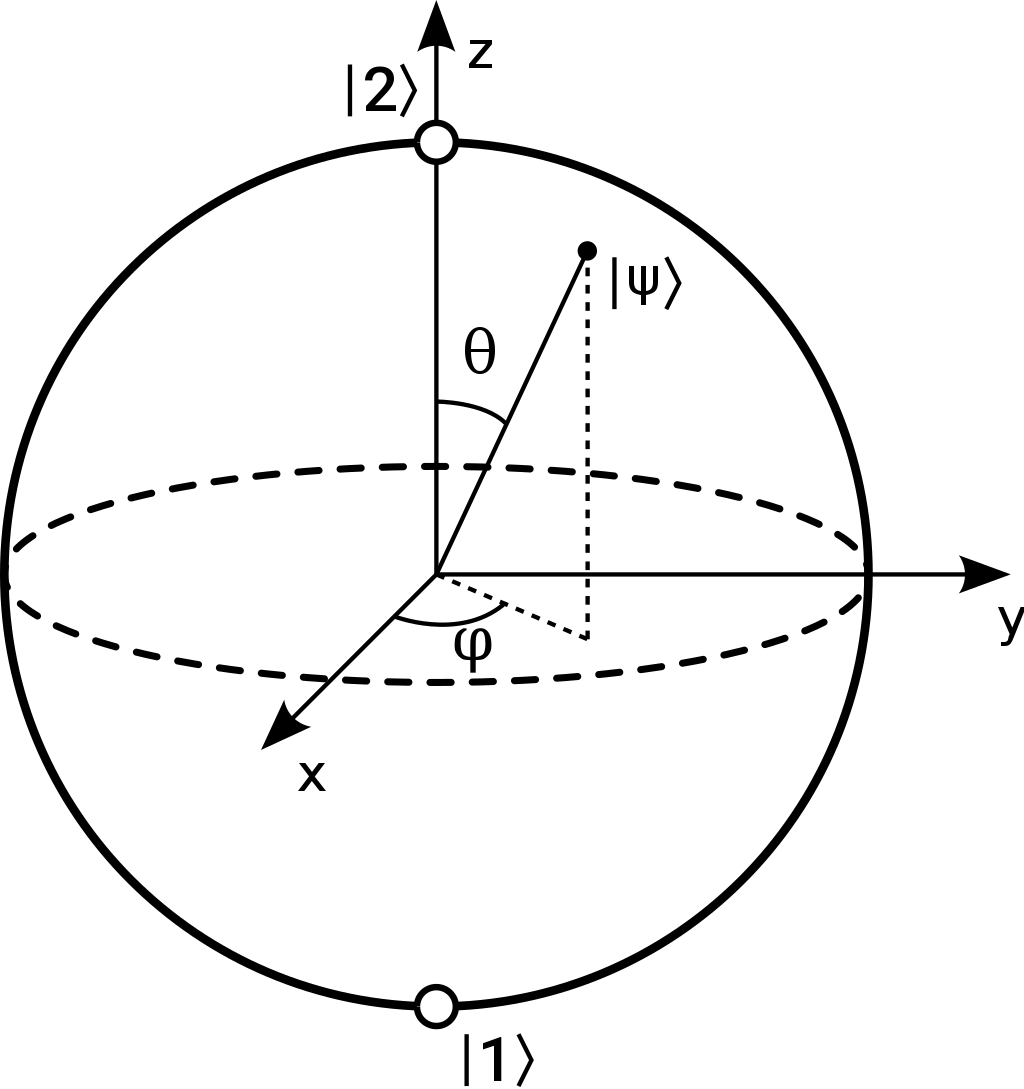
\includegraphics[width=0.35\textwidth]{USPSC-img/Bloch_sphere.png}
		\legend{Bloch sphere for a pure state given by \\ $ \ket{\psi} = \sin(\theta/2) \ket{1} + e^{i\phi} \cos(\theta/2) \ket{2} $. \\ Source: Author}
		\label{fig:Bloch-sphere}
		\vspace{-5pt}
	\end{wrapfigure}
	Let us consider a pure state $ \ket{\psi} = c_1\ket{1} + c_2\ket{2} $. Since a global phase is not measurable, we can assume $ \ket{\psi} = c_1 \ket{1} + c_2 e^{i\phi} \ket{2} $ where $ \phi $ is the phase difference between $ \ket{1} $ and $ \ket{2} $, and both $ c_1 $ and $ c_2 $ are real values. Moreover, $ c_1^2 + c_2^2 = 1 $, which allows us to associate $ c_1 $ and $ c_2 $ with a unique value $ \theta $ considering $ c_1 = \sin{(\theta/2)} $ and $ c_2 = \cos{(\theta/2)} $. Even though the value of $ \theta $ is not unique to represent $ c_1 $ and $ c_2 $, the point $ (\theta, \phi) $ is unique to represent $ \ket{\psi} $. Thus, a density operator $ \hat{\rho} = \ketbra{\psi}{\psi} $ of a pure state can be written as
	\begin{align}
		\hat{\rho} &= \sin^2(\theta/2) \ketbra{1}{1} + \cos^2(\theta/2) \ketbra{2}{2} + \nonumber 
		\\
		&+ \frac{1}{2}e^{-i\phi}\sin\theta \ketbra{1}{2} + \frac{1}{2}e^{i\phi}\sin\theta \ketbra{2}{1},
	\end{align}
\end{minipage}

\begin{equation}
	\hat{\rho} = \left[ \begin{matrix} \sin^2(\theta/2) & \frac{1}{2}e^{-i\phi}\sin\theta \\ \frac{1}{2}e^{i\phi}\sin\theta & \cos^2(\theta/2) \end{matrix} \right].
	\label{eq:density-matrix-pure-state-spherical-coordinates}
\end{equation}
From equations (\ref{eq:density-matrix-on-Pauli-basis}) and (\ref{eq:density-matrix-pure-state-spherical-coordinates}), we obtain the following Bloch vector
\begin{equation}
	\mathbf{a} = (\cos\phi \sin\theta, \sin\phi \sin\theta, \cos\theta),
\end{equation}
in which $ (\phi, \theta) $ are \textit{spherical coordinates} represented in figure \ref{fig:Bloch-sphere}.

%
%-----------------------------------
\subsection{Liouville equation}
\label{sec:Liouville-equations}
%-----------------------------------
%

The time evolution of a state vector $ \ket{\psi} $ is given by the Schrodinger equation $ \hat{H} \ket{\psi} = i \hbar \partial_t \ket{\psi} $, where $ \hat{H} $ is the Hamiltonian of the system. Thereby, the time evolution of $ \hat{\rho} $ is given by
\begin{align}
	\partial_t \hat{\rho} &= \partial_t \left( \sum_{k} P_k \ketbra{\psi_k}{\psi_k} \right) = \sum_{k} P_k [(\partial_t \ket{\psi_k})\bra{\psi_k} + \ket{\psi_k}(\partial_t \bra{\psi_k})] = \\
	&= \frac{i}{\hbar} \sum_{k} P_k (\ketbra{\psi_k}{\psi_k} \hat{H} - \hat{H}\ketbra{\psi_k}{\psi_k}) = \hat{\rho}\hat{H} - \hat{H}\hat{\rho}
\end{align}
Therefore,
\begin{equation}
	\partial_t \hat{\rho} = \frac{i}{\hbar} [\hat{\rho}, \hat{H}],
	\label{eq:Liouville-equation}
\end{equation}
where the equation (\ref{eq:Liouville-equation}) is called \textbf{von Neumann equation} or \textbf{Liouville equation}. The commutator itself can be considered as a \textbf{superoperator} acting on the density operator,
\begin{equation}
	\mathcal{L}\hat{\rho}(t) \equiv - \frac{i}{\hbar} [\hat{H}, \hat{\rho}(t)],
	\label{eq:Liouville-superoperator}
\end{equation}
where $ \mathcal{L} $ is known as \textbf{Liouville superoperator}. We shall work with a Hamiltonian in the form $ \hat{H} = \hat{H}_0 + \hat{V}(t) $, where $ \hat{H}_0 $ is a time-independent part and $ \hat{V}(t) $ is a time-dependent term. In this case, it is convenient to define an unitary transformation given by $ \hat{U}(t) = e^{- i \hat{H}_0 t / \hbar} $ so that 
\begin{equation}
	\hat{\rho}'(t) = \hat{U}^{\dagger}(t)\hat{\rho}(t)\hat{U}(t).
	\label{eq:density-operator-interaction-picture}
\end{equation}
Calculating the time derivatives on both sides of (\ref{eq:density-operator-interaction-picture}) and assuming (\ref{eq:Liouville-equation}), we obtain
\begin{equation}
	\partial_t \hat{\rho}'(t) = - \frac{i}{\hbar} [\hat{V}(t), \hat{\rho}'(t)].
	\label{eq:von-Neumann-equation-interaction-picture}
\end{equation}
The equation (\ref{eq:von-Neumann-equation-interaction-picture}) is the \textbf{Liouville equation} in the \textbf{interaction picture}, which depends only on the time-dependent part.

The equation (\ref{eq:Liouville-equation}) is valid as long as there are only coherent effects on the system,  since these processes are represented by unitary time evolutions\footnote{An unitary time evolution is associated with a hermitian Hamiltonian so that $ \hat{U} = e^{-i \hat{H}t / \hbar} $.}. In the context of atom-light interaction when we assume an density operator associated with the atomic internal states, the Liouville equation only describes stimulated absorption and emission. However, spontaneous emission is a predominant process in MOTs, so it is mandatory to take it into account. In order to comply with that, we shall introduce the \textit{master equation} in section \ref{sec:master-equation}.

%
%-----------------------------------
\subsection{Master equation}
\label{sec:master-equation}
%-----------------------------------
%

Spontaneous emission comes from a coupling between an open quantum system, described by the density operator $ \hat{\rho}_S $, and the environment, represented by the density operator $ \hat{\rho}_E $. Moreover, the environment must have far more degrees of freedom than the system. In our case, the system can be understood as the atom and the environment as the vacuum modes of the quantized electromagnetic field. Let us consider a density operator $ \hat{\rho}_{SE} $ which represents jointly the system and the environment. Assuming a weak coupling in which the system performs a small perturbation to the environment, we can treat both independently so that
\begin{equation}
	\hat{\rho}_{SE} \approx \hat{\rho}_S \otimes \hat{\rho}_E.
	\label{eq:Born-approximation}
\end{equation}
The equation (\ref{eq:Born-approximation}) is known as the \textbf{Born approximation}. At first, both system and environment provoke mutual excitations, getting out of thermal equilibrium. After a while, both will reach equilibrium again through a relaxation process. Let us consider the relaxation times $ \tau_E $ and $ \tau_S $ of the environment and the system, respectively. Since the system causes small perturbation to the environment but the environment interacts strongly with the system, we can consider $ \tau_E \ll \tau_S $. This is known as \textbf{Markov approximation}. The equation of motion of $ \hat{\rho}_{SE} $ is given by the Liouville equation,
\begin{equation}
	i \hbar \partial_t \hat{\rho}_{SE} = [\hat{H}_{SE}, \hat{\rho}_{SE}].
	\label{eq:Liouville-equation-system-environment}
\end{equation}
Let us consider a multi-level system given by the basis $\{\ket{n}\}$. Taking the Born-Markov approximation into account, it is possible to derive an equation of motion for $ \hat{\rho}_S $ tracing out the environment in equation (\ref{eq:Liouville-equation-system-environment}). The resulting equation \cite{brasil2013simple}, known as \textbf{master equation} or \textbf{Lindblad equation}, is given by
\begin{gather}
	\partial_t \hat{\rho}_S = \frac{1}{i\hbar} [\hat{H}_S, \hat{\rho}_S] + \sum_{i,j} \frac{\Gamma_{ij}}{2}(2\hat{\sigma}_{ij}\hat{\rho}_{S}\hat{\sigma}_{ji} - \{\hat{\sigma}_{ji}\hat{\sigma}_{ij}, \hat{\rho}_{S}\}) = (\mathcal{L} + \mathcal{L}_{decay}) \hat{\rho}_S,
	\label{eq:Lindblad-equation}
	\\
	\mathcal{L}_{decay}\hat{\rho} = \sum_{i,j} \frac{\Gamma_{ij}}{2}(2\hat{\sigma}_{ij}\hat{\rho}_{S}\hat{\sigma}_{ji} - \{\hat{\sigma}_{ji}\hat{\sigma}_{ij}, \hat{\rho}_{S}\}),
	\label{eq:Lindblad-superoperator}
\end{gather}
where $ \hat{\sigma}_{ij} = \ketbra{i}{j} $, $ \mathcal{L}_{decay} $ is the \textbf{Lindblad superoperator}, $ \{\hat{A}, \hat{B}\} = \hat{A}\hat{B} + \hat{A}\hat{B}$ is the anticommutator, and $ \{\Gamma_{i,j}\} $ are rates, known as \textit{decay rates}, at which both populations and coherences vanish. The operators $ \hat{\sigma}_{i,j} $ and $ \hat{\sigma}_{j,i} = \hat{\sigma}_{i,j}^{\dagger} $ can be understood as \textit{lower} and \textit{upper operators} between the states $ \ket{i} $ and $ \ket{j} $ so that $ \hat{\sigma}_{i,j} \ket{j} = \ket{i} $ and $ \hat{\sigma}_{j,i} \ket{i} = \ket{j} $. The master equation results in the Liouville equation when $ \Gamma_{ij} \longrightarrow 0,\ \forall i,j $. Therefore, the difference between these equations is the decay term expressed by the superoperator $ \mathcal{L}_{decay} $ known as \textbf{Lindblad superoperator}.

Let us consider the case in which only $ \{\Gamma_{i,i} = \Gamma_i \} $ are non-zero. Then, the superoperator $ \mathcal{L}_{decay} $ can be written as
\begin{equation}
	\mathcal{L}_{decay} \hat{\rho} = - \frac{1}{2} \sum_{i} \Gamma_i \left( \sum_{j \neq i} \rho_{i,j} \ketbra{i}{j} + \sum_{k \neq i} \rho_{k,i} \ketbra{k}{i} \right),
	\label{eq:decay-superoperator-dephasing}
\end{equation}
where $ \rho_{i,j} \equiv \braket{i|\hat{\rho}|j} $. From equation (\ref{eq:decay-superoperator-dephasing}), it is possible to see that only the off-diagonal terms are affected by $ \mathcal{L}_{decay} $. Hence, only the coherences decay since they are associated with the off-diagonal terms. This process is known as \textbf{pure dephasing}. In the general case when $ \Gamma_{i,j} > 0 $ for $  i \neq j $, the populations also change over time, which is known as \textbf{relaxation}. Spontaneous emission is only responsible for \textit{relaxation} terms $ \{ \Gamma_{i,j},\ i \neq j,\ i  < j \} $, whereas the \textit{pure dephasing} terms $ \{ \Gamma_{i} \} $ are associated with \textbf{elastic collisions}. Furthermore, $\{ \Gamma_{i} \} $ are the rates at which the atoms collide between each other. We are concerned only with the regime of low temperatures in which collisions are negligible.